\chapter{Tricks}
\section{Dropout}
\subsection{Dropout}
The key idea is to randomly drop units (along with their connections) from the neural
network during training\cite{DropOut2012,Srivastava2014}.
\begin{figure}[H]
    \centering
    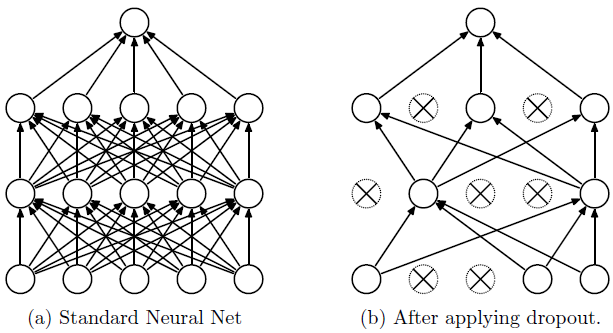
\includegraphics[width=12cm]{images/dropout.png}
    \caption{Dropout Neural Net Model. 
    \textbf{Left}: A standard neural net with 2 hidden layers. 
    \textbf{Right}:An example of a thinned net produced by applying dropout to the network on the left. Crossed units have been dropped.}
    \label{fig:dropout}
\end{figure}

\subsection{DropConnect}
DropConnect\cite{Wan2013} instead sets a randomly selected subset of weights within the network to zero.

\subsubsection{Stochastic Depth}
The gradients can vanish, the forward flow often diminishes, and the training time can be painfully slow. 
To address these problems, we propose \textbf{stochastic depth}, a training procedure that enables
the seemingly contradictory setup to \textit{train short} networks and \textit{use deep} networks at test time. 
We start with very deep networks but during training, for each mini-batch, randomly drop a subset of layers and bypass
them with the identity function.

To reduce the effiective length of a neural network during training, 
we \textbf{randomly skip layers entirely}. 
We achieve this by introducing skip connections in the same fashion as ResNets, 
however the connection pattern is \textit{randomly altered for each mini-batch}.

\subsubsection{Stochastic depth during testing} 
However, during training, functions $f_l$ are only active for a fraction $p_l$ of all updates, 
and the corresponding weights of the next layer are calibrated for this survival probability. 
\textbf{We therefore need to re-calibrate the outputs of any given function $f_l$ by the expected number of times
it participates in training, $p_l$.} The forward propagation update rule becomes:
\[
    H_l^{test} = ReLU(p_l f_l(H^{test}_{l-1}; W_l) + H^{test}_{l-1})
\]

\subsubsection{The survival probabilities}
$p_l$

\section{Augment}
\section{SpeedUp}
\begin{itemize}
    \item \textbf{progressive learning}: in the early training epochs, we train the
    network with small image size and weak regularization (e.g., dropout and data augmentation),
    then we gradually increase image size and add stronger regularization.
    \item 
\end{itemize}